\documentclass[../main.tex]{subfiles}

\begin{document} %%%%%%%%%%%%%%%%%%%%%%%%%%%%%%%%%%%%%%%%%%%%%%%%%%%%%%%%%%%%
\section{Algoritmo simplex} 
    El algoritmo simplex se usa para resolver PL que tienen muchas variables y restricciones.
    
    \subsection{Convertir un PL en forma estandar}
        \begin{definition} \textbf{(PL forma estándar)}
            Un PL está en forma estándar si:
            \begin{itemize}
                \item Las restricciones son de igualdad.
                \item Las variables de decisión son no negativas.
            \end{itemize}
        \end{definition}

        \begin{example} \textbf{(Leather Limited)}\\
            
        \end{example}

    \subsection{Preliminares del algoritmo simplex}
        Suponga que se ha convertido un PL con $m$ restricciones en su forma estándar. Si se supone que la forma estándar contiene $n$ variables (denominadas por conveniencia $x_1, x_2, \dots, x_n$), la forma estándar para tal PL es
        \begin{equation}
            \max o \min(z) = c_1 \cdot x_1 + c_2 \cdot x_2 + \dots + c_n \cdot x_n
        \end{equation}

        sujeto a
        \begin{equation}
            \begin{aligned}
                a_{11} \cdot x_1 + a_{12} \cdot x_2 + \dots + a_{1n} \cdot x_n &= b_1 \\
                a_{21} \cdot x_1 + a_{22} \cdot x_2 + \dots + a_{2n} \cdot x_n &= b_2 \\
                \vdots \\
                a_{m1} \cdot x_1 + a_{m2} \cdot x_2 + \dots + a_{mn} \cdot x_n &= b_m \\
                x_1, x_2, \dots, x_n &\geq 0 \\
            \end{aligned}
            \label{eq:forma_estandar}
        \end{equation}

        Se define matriz
        \begin{equation}
            A = \begin{bmatrix}
                a_{11} & a_{12} & \dots & a_{1n} \\
                a_{21} & a_{22} & \dots & a_{2n} \\
                \vdots & \vdots & \ddots & \vdots \\
                a_{m1} & a_{m2} & \dots & a_{mn} \\
            \end{bmatrix}
        \end{equation}

        y
        \begin{equation}
            x = \begin{bmatrix}
                x_1 \\
                x_2 \\
                \vdots \\
                x_n \\
            \end{bmatrix}, \quad 
            b = \begin{bmatrix}
                b_1 \\
                b_2 \\
                \vdots \\
                b_m \\
            \end{bmatrix} \quad
        \end{equation}


    \subsection{Variables básicas y no básicas}
        Con el sistema $A \cdot x = b$ de $m$ ecuaciones lineales y $n$ variables (suponga $n \geq m$).

        \begin{definition} \textbf{(Solucion básica)}
            Una solucion básica para $A \cdot x = b$ se obtiene haciendo $n-m$ variables iguales a cero, y luego se determinan los valores de las $m$ variables restantes. Así se asume que al hacer las $n-m$ variables iguales a cero se llega a valores únicos para las $m$ variables restantes, o que, en forma equivalente, las columnas para las $m$ variables restantes son linealmente independientes.
        \end{definition}

        \begin{enumerate}
            \item Escoger un conjuto de $n-m$ variables no básicas (VNB).
            \item Igualar a cero las vaariables no básicas.
        \end{enumerate}

        \begin{definition} \textbf{(Puntos esquina)}
            Una solución básica es un punto esquina si todas las variables son no negativas.
            
            La cantidad máxima de puntos esquina es 
            \begin{equation}
                C^n_m = \binom{n}{m} = \frac{n!}{m! \cdot (n-m)!}
            \end{equation} 
            
        \end{definition}

        \begin{example}
            \begin{equation}
                \begin{aligned}
                    x_1 + x_2 &= 3 \\
                    - x_2 + x_3 &= -1 \\
                \end{aligned}
            \end{equation}

            Variables no básicas (VNB): $n-m = 3-2 = 1$.
            \begin{table}[h]
                \begin{center}
                    \begin{tabular}{|c|c|c|}
                        \hline
                        VNB $= {x_3}$, BV $= \{x_1,x_2\}$ & VNB $= {x_2}$, BV $= \{x_1,x_3\}$ & VNB $= {x_1}$, BV $= \{x_2,x_3\}$ \\ \hline
                        $x_3 = 0$ & $x_2 = 0$ & $x_1 = 0$ \\ \hline
                        \begin{minipage}{.3\textwidth}
                            \begin{equation*}
                                \begin{aligned}
                                    x_1 + x_2 &= 3\\
                                    x_2 &= -1 \\
                                \end{aligned}
                            \end{equation*}
                        \end{minipage} & \begin{minipage}{.3\textwidth}
                            \begin{equation*}
                                \begin{aligned}
                                    x_1 &= 3\\
                                    x_3 &= -1 \\
                                \end{aligned}
                            \end{equation*}
                        \end{minipage} & \begin{minipage}{.3\textwidth}
                            \begin{equation*}
                                \begin{aligned}
                                    x_2 &= 3\\
                                    -x_2 +x_3 &= -1 \\
                                \end{aligned}
                            \end{equation*}
                        \end{minipage} \\ \hline
                        $x_1 = 2, x_2 = 1, x_3 = 0$ & $x_1 = 3, x_2 = 0, x_3 = -1$ & $x_1 = 0, x_2 = 3, x_3 = 2$ \\ \hline
                    \end{tabular}
                \end{center}
                \caption{Soluciones básicas}
            \end{table}
            \label{table:ejemplo_soluciones_básicas}
        \end{example}
        
    \subsection{Soluciones factibles}    
        \begin{definition} \textbf{(solución básica factible (sbf))}
            Cualquier solucion básica de (\ref{eq:forma_estandar}) en la cual todas las variables son no negatiavas.
        \end{definition}

        \begin{definition} \textbf{(punto estremo)}
            Un punto en la región factible de un PL es un punto extremo si y sólo si es una solución factible básica. 
        \end{definition}

        \begin{example}
            Ejemplo sacado del libro Hamby A Taha pág 73.
            \begin{equation}
                \min Z = 2 \cdot x_1 + 3 \cdot x_2
            \end{equation}

            sujeto a
            \begin{equation}
                \begin{aligned}
                    x_1 + x_2 &\leq 4 \\
                    x_1 + 2 \cdot x_2 &\leq 5 \\
                    x_1, x_2 &\geq 0 \\
                \end{aligned}
            \end{equation}

            \begin{table}[h]
                \centering
                \begin{tabular}{cccccc}
                \hline
                \multirow{2}{*}{\textbf{\begin{tabular}[c]{@{}c@{}}Variables no\\ básicas (cero)\end{tabular}}} & \multirow{2}{*}{\textbf{Variables básicas}} & \multirow{2}{*}{\textbf{Solución básica}} & \multirow{2}{*}{\textbf{\begin{tabular}[c]{@{}c@{}}Punto de esquina\\ asociado\end{tabular}}} & \multirow{2}{*}{\textbf{¿Factible?}} & \multirow{2}{*}{\textbf{\begin{tabular}[c]{@{}c@{}}Valor\\ objetivo, z\end{tabular}}} \\
                &&&&&\\ \hline
                $(x_1,x_2)$ & $(s_1,s_2)$ & (4,5) & A & Sí & 0 \\
                $(x_1,s_1)$ & $(x_2,s_2)$ & (4,-3)& F& No& -\\
                $(x_1,s_2)$ & $(x_2,s_1)$ & (2.5,1.5)& B& Sí& 7.5\\
                $(x_2,s_1)$ & $(x_1,s_2)$ & (2,3)& D& Sí& 4\\
                $(x_2,s_2)$ & $(x_1,s_1)$ & (5,-6)& E& No& -\\
                $(s_1,s_2)$ & $(x_1,x_2)$ & \textbf{(1,2)}& \textbf{C}& \textbf{Sí}& \textbf{8 (óptimo) }\\
                \hline
                \end{tabular}
                \caption{Soluciones básicas}
            \end{table}

            % Carganos imagen
            \begin{figure}[h]
                \centering
                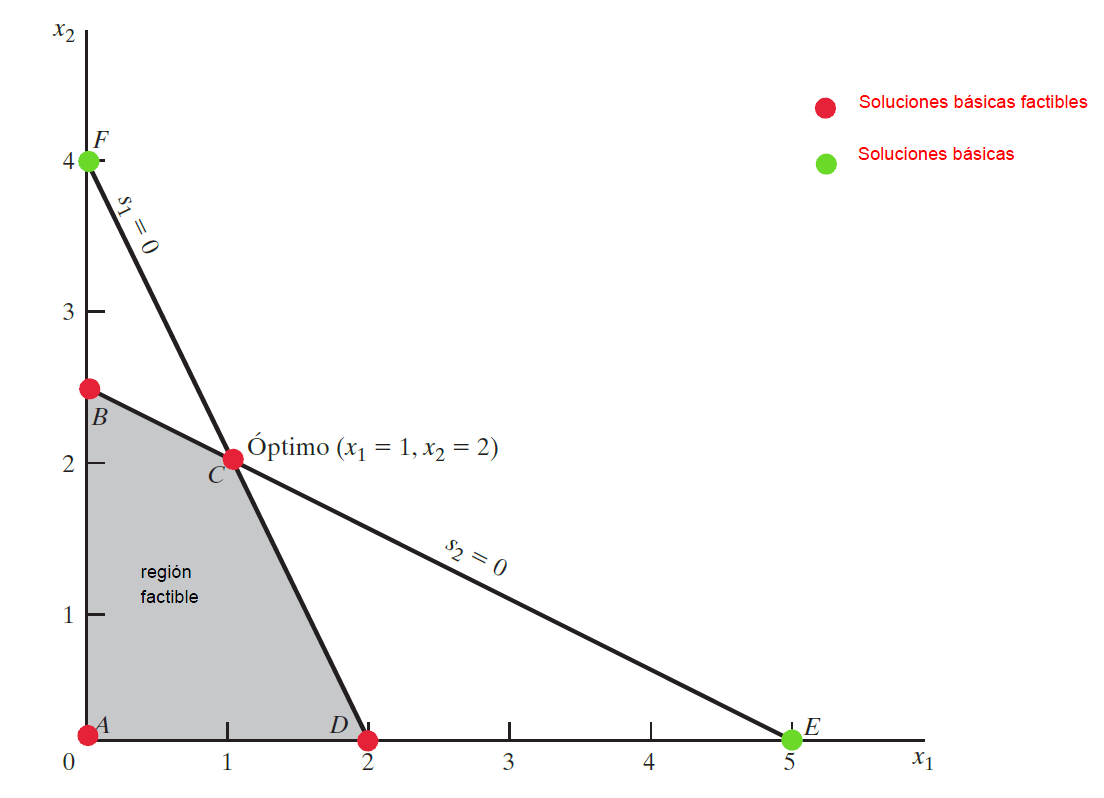
\includegraphics[width=0.7\textwidth]{../images/variable_basicas.png}
                \caption{Región factible}
                \label{fig:region_factible}
            \end{figure}

            Las soluciones básicas estan conformadas por $(x_1, x_2, s_1, s_2)$. Por ejemplo $A=(0,0,4,5)$, y es factible si todas sus variables son positivas.
        \end{example}
        

    \subsection{Álgebra del método símplex}
        \begin{example} Ejemplo tomado del video YouTube \cite{metodo_simplex_algebraico}.
            \begin{equation}
                \max z = 7 \cdot x_1 + 4 \cdot x_2
            \end{equation}

            sujeto a
            \begin{equation}
                \begin{aligned}
                    2 \cdot x_1 + x_2 &\leq 20 \\
                    x_1 + x_2 &\leq 18 \\
                    x_1  &\leq 8 \\
                    x_1, x_2 &\geq 0 \\
                \end{aligned}
            \end{equation}

            \underline{\textbf{Solución:}}
            \begin{enumerate}
                \item  Forma estándar o aumentada:
                    \begin{equation}
                        \begin{aligned}
                            2 \cdot x_1 + x_2 + s_1 &= 20 \\
                            x_1 + x_2 + s_2 &= 18 \\
                            x_1 + s_3 &= 8 \\
                            x_1, x_2, s_1, s_2, s_3 &\geq 0 \\
                        \end{aligned}
                    \end{equation}
                    
                    Tenemos $m = 3$ restricciones y $n = 5$ variables. Por lo tanto, $n-m = 2$ variables no básicas y $m = 3$ variables básicas.

                    Si $x_1 = x_2 = 0$, entonces $s_1 = 20$, $s_2 = 18$ y $s_3 = 8$. Por lo tanto, $(0,0,20,18,8)$ es una solución básica factible.
                \item Determinación de la dirección de movimiento.
 
                    Observando la funcion objetivo $z$ aumenta más rápidamente si $x_1$ aumenta en una unidad. Por lo tanto, $x_1$ es la variable de entrada.
                    \begin{equation}
                        \begin{aligned}
                            \text{¿Aumenta $x_1$?} && \text{Tasa de mejoramiento} && z &= 7 \\
                            \text{¿Aumenta $x_2$?} && \text{Tasa de mejoramiento} && z &= 4 \\
                        \end{aligned}
                    \end{equation}

                    Con esto se determina la variable de entrada $x_1$.

                \item Prueba del cociente mínimo.
                    Cuanto aumentar el valor de la variable básica entrante $x_1$ antes de detenerse, para no salirse de la región factible.

                    En la primer ecuación se observa que el valor más pequeño que tomar la variable $s_1 = 0$. Seguimos asi con el razonamiento para las demás ecuaciones.

                    Usando las restricciones y sabiendo que $x_2 = 0$, se obtiene:
                    \begin{equation}
                        \begin{aligned}
                            2 \cdot x_1 + s_1 &= 20 && (x_1 \leq 10)\\
                            x_1 + s_2 &= 18 && (x_1 \leq 18)\\
                            x_1 + s_3 &= 8 && (x_1 \leq 8) && \leftarrow \text{mínimo}\\
                            x_1, s_1, s_2, s_3 &\geq 0 \\
                        \end{aligned}
                    \end{equation}

                    Se la restricción que más limita el crecimiento se despeja y se la coloca en las demás ecuaciones.
                \item Resolución de una nueva solución BF.
                    Se reemplaza $x_1 = 8 - s_3$ en las demás ecuaciones:
                    \begin{equation}
                        \begin{split}
                            \max z &= 7 \cdot (8 - s_3) + 4 \cdot x_2 \\
                                   &= 56 + 4 \cdot x_2 - 7 \cdot s_3 \\
                        \end{split}
                    \end{equation}

                    \begin{equation}
                        \begin{aligned}
                          2 \cdot (8 - s_3) + x_2 + s_4 &= 20 && \longrightarrow && x_2 + s_1 -2 \cdot s_3 = 4 \\
                            (8 - s_3) + x_2 + s_4 &= 18 && \longrightarrow && x_2 + s_2 - s_3 = 10 
                        \end{aligned}
                    \end{equation}

                    El sistema de ecuaciones equivalente es
                    \begin{equation}
                        \begin{split}
                            \max z &= 56 + 4 \cdot x_2 - 7 \cdot s_3 \\
                        \end{split}
                    \end{equation}

                    \begin{equation}
                        \begin{aligned}
                          x_2 + s_1 -2 \cdot s_3 = 4 \\
                          x_2 + s_2 - s_3 = 10 \\
                          x_1 + s_3 = 8 \\
                            x_1, x_2, s_1, s_2, s_3 &\geq 0 \\
                        \end{aligned}
                    \end{equation}
                \item Una vez que se tiene un sistema de ecuaciones equivalente, se repite el proceso.
                    
                    Una forma fácil de identificar que variables se ponen en cero se observa la función objetivo $x_2 = 0$ y $s_3 = 0$.

                    Otra forma es observando el sistema de ecuaciones y ver las variables con coeficiente uno.
                \item Prueba del cociente mínimo.
                
                    Como $s_3=0$, se obtiene:
                    \begin{equation}
                        \begin{aligned}
                            x_2 + s_1 &= 4 && (x_2 \leq 4) && \leftarrow \text{mínimo} \\
                            x_2 + s_2 &= 10 && (x_2 \leq 10)\\
                            x_1 &= 8 &&  && \leftarrow \text{sin restricción}\\
                            x_1, x_2, s_1, s_2, s_3 &\geq 0 \\
                        \end{aligned}
                    \end{equation}

                    Se la restricción que más limita el crecimiento se despeja y se la coloca en las demás ecuaciones.
                \item Resolución de una nueva solución BF.
                
                    Despejando de la primer ecuación:
                    \begin{equation}
                        x_2 + s_1 -2 \cdot s_3 = 4 \quad \longrightarrow \quad x_2 = 4 - s_1 + 2 \cdot s_3
                    \end{equation}

                    Reemplamos en todo el sistema equivalente:
                    \begin{equation}
                        \begin{aligned}
                        \max z &= 56 + 4 \cdot (4 - s_1 + 2 \cdot s_3) - 7 \cdot s_3 \\
                               &= 72 - 4 \cdot s_1 - s_3 \\
                        \end{aligned}
                    \end{equation}

                    \begin{equation}
                        \begin{aligned}
                          (4 - s_1 + 2 \cdot s_3) + s_2 - s_3 &= 10 && \longrightarrow && -s_1 + s_2 + s_3 = 6 \\
                        \end{aligned}
                    \end{equation}


                    El sistema equivalente queda:
                    \begin{equation}
                        \begin{aligned}
                        \max z &= 72 - 4 \cdot s_1 - s_3 \\
                        x_2 + s_1 -2 \cdot s_3 &= 4 \\
                          -s_1 + s_2 + s_3 &= 6 \\
                          x_1 + s_3 &= 8 \\
                            x_1, x_2, s_1, s_2, s_3 &\geq 0 \\
                        \end{aligned}
                    \end{equation}
                \item Seguimos asi.
            \end{enumerate} 
        \end{example}



































































\end{document}  %%%%%%%%%%%%%%%%%%%%%%%%%%%%%%%%%%%%%%%%%%%%%%%%%%%%%%%%%%%%%
